% !TeX root = ../main.tex

\chapter{实验数据}
实验数据一方面来源于真实的质子--质子碰撞事件,另一方面来源于蒙特卡洛(MC)模拟。
分析通过模拟期望的超越标准模型(BSM)的物理过程,得到该过程在探测器中的事件特征,并通过机器学习算法学习提取特征,
之后将提取到的特征与真实数据进行比较,以期得到新物理存在的证明。

\section{数据来源}

\subsection{探测器数据}
\label{sec:detector_data}

分析所用的数据集是在2015年至2018年期间,由ATLAS探测器通过LHC上质子--质子($pp$)碰撞($\sqrt{s} = 13\,\mathrm{TeV}$)收集的。
该数据集的总积分亮度为 $140\,\mathrm{fb}^{-1}$。排除了LHC束流不稳定或并非所有子探测器都在运行的数据~\cite{ATLAS_data_quality}。

ATLAS 探测器使用分层触发系统记录事件。
一级 (L1) 触发器采用定制电子设备实现,可将事件发生率从 LHC 束流交汇频率 40~MHz 降低到设计值 100~kHz。
第二级触发器称为高级触发器 (HLT),由运行在商用计算机集群上的软件实现,该软件可处理事件并将记录事件的发生率降低到 1 kHz。
软件套件用于数据模拟、真实数据和模拟数据的重建和分析、探测器操作以及实验的触发和数据采集系统。


\subsubsection{信号数据}
本分析依据最终态的物理对象将信号分为三个通道进行研究,
这三类通道分别针对 LLP 的不同产生机制与动量范围,实现了信号覆盖范围的互补性:
\begin{itemize}
    \item {CalRatio + 双喷注(CalR+2J):} 该通道主要针对隐藏区域(Hidden Sector, HS)模型中介子粒子的胶子–胶子融合($gg \to \Phi$)产生模式,
          中介粒子再衰变到一对长寿命粒子($\Phi \to ss$)后其中一个$s$具有足够短的衰变长度与动量,使其在探测器中产生两个可分辨的位移喷注。

    \item {CalRatio + W玻色子(CalR+W):} 该通道目标为伴随 $W$ 玻色子产生 LLP 的情形,
          如 HS 模型中介子粒子伴随 $W$ 玻色子产生,或类轴轻子(Axion-like Particle, ALP)从 $W$ 玻色子辐射而来。
          通过选取 $W$ 的轻子衰变产物(电子或 $\mu$ 子)增强触发效率并抑制背景。

    \item {CalRatio + Z玻色子(CalR+Z):} 类似于 CalR+W 通道,CalR+Z 通道利用 $Z$ 玻色子的轻子衰变作为分析入口,
          适用于 LLP 与 $Z$ 玻色子共同产生的场景,如 ALP 或暗光子模型中 $Z$ 联合产生机制。
\end{itemize}

为了获取符合信号特征的数据,对于CalRatio+2J通道,分析使用了专门的LLP触发器,称为CalRatio触发器。
在一级触发阶段,喷注在 $\eta \times \phi$ 平面中的 $0.2 \times 0.2$ 区域进行重建,这是基于信号喷注通常比标准模型喷注更窄的事实。
选取的事件要求喷注的横能量 $E_T$ 超过 60~\GeV 或 100~\GeV(具体取决于数据收集时期)。
在某些运行阶段,存在一些触发器,其要求仅在喷注所在的 $\eta - \phi$ 位置上电磁量能器中没有能量沉积时才接受L1喷注对象。
该要求可作为 CalRatio 指标的替代,使得 $E_T$ 阈值可降低至 30~\GeV。

在高级触发阶段,触发喷注还需满足 $|\eta| < 2.5$ 的条件,即在可获得径迹信息的范围内。
此外,该喷注还应具有高比例的强子量能器能量沉积,并满足修改后的噪声抑制条件,
并通过一种用于去除束流背景(Beam Induced Background,BIB)的算法(例如利用能量沉积在 $\phi$ 方向上的时间和对准信息)。
在其余通道中,使用了单轻子或双轻子触发器,仅考虑在某一年中整个数据收集期间未进行舍选的触发器。


\subsubsection{背景数据}
为研究非碰撞背景(NCB)以及构建验证区和控制区,额外收集了三个数据集:
BIB 数据集包含满足 CalRatio 触发器所有要求但未通过 BIB 去除算法的事件。
宇宙射线数据集使用相同的触发器选择标准,但来自空束团交叉(bunch-crossing, BC)期间记录的事件。
双喷注(dijet)数据集是通过基于单喷注触发器~\cite{trigger} 的触发器选择的,并排除了 CalRatio 触发器,从而确保其与主数据集正交。
该数据集用于测试位移喷注(displaced jet)神经网络标注器(neural network tagger)输出中建模的影响。

源自束流背景(BIB)的粒子可能在量能器中产生喷注,但在电磁量能器(ECal)或内径迹探测器中不产生任何信号。
在这种情况下,所产生的喷注将具有与真实 CalRatio 喷注非常相似的特性。
如上所述,触发器需要包含一个用于排除 BIB 的算法,但该算法只能识别具有负时间的假喷注。
来自下一个束团交叠的 BIB 事件可能会产生具有正时间的假喷注,从而通过主要触发条件。

满足上述所有条件的喷注还需通过一个基于探测器单元时间与位置的 BIB 抑制算法。
BIB 是由束晕(beam-halo)或束气(beam-gas)效应在探测器中产生的μ子组成的,这些μ子与质子束同步传播,并平行于束管方向。
在 BIB 中,由μ子在强子量能器(HCal)中沉积能量所产生的喷注可能会伪装为信号喷注,从而被 CalRatio 触发器接受。

该BIB抑制算法利用了以下事实:由 BIB 产生的量能器击中位置(hit)通常沿着一条相对水平、平行于束管的直线分布,并且具有特定的时间分布特征,
这些特征与从相互作用点(IP)出发以光速传播到击中位置所需时间并不一致。
当在与触发喷注在相同的 $\phi$ 处、但在 $\Delta R$ 上有一定间隔的位置上,
存在至少四个探测单元的时间一致且与当前束团交叠中 BIB μ子的时间一致时,该算法将拒绝该事件。
此处的 BIB μ子是指以光速传播、通过端盖区域进入量能器、与质子束同步但沿水平方向传播的粒子。
关于算法的详细描述见文献~\cite{ATLAS-CONF-2016-103} 的附录 B。

需要指出的是,算法中对 BIB 探测单元时间的要求为 $t < -2\,\mathrm{ns}$,
这使其在排除当前束团交叠(BC)中的 BIB 方面较为有效,但对于来自下一个或下下个束团交叉的 BIB 则无能为力。
此类 BIB 仍可能通过主 CalRatio 触发器,从而污染标准选区。
因此,需要应用 BDT 以进一步抑制 BIB 对分析的影响。


\subsection{模拟数据}
\label{sec:MC}

\subsubsection{信号数据}
本分析总计考虑三种基准信号模型。第一种是隐藏区域(HS)模型,其中标量玻色子 $\Phi$(可以是希格斯玻色子,
也可以是其他行为类似的较轻或较重粒子)作为标准模型与隐藏区域之间的媒介。
$\Phi$ 可衰变为中性的长寿命标量粒子 $S$,通常衰变为运动学允许的最重费米子对,通常为 $b$ 夸克对。
事件使用 \MADGRAPH{5\_aMC@NLO v2.6.2}~\cite{Alwall:2014hca} 在 LO 精度下生成,使用 NNPDF2.3LO PDF 集。
考虑 $\Phi$ 的两种产生模式:CalR+2J 通道中为胶子--胶子融合(ggF),CalR+W/Z 通道中为伴随矢量玻色子(W 或 Z)产生。
在 CalR+2J 通道中,所有选择对象均来源于 LLP 的衰变,没有预期来自矢量玻色子融合(VBF)模式的显著贡献。
伴随 W 或 Z 玻色子产生的 HS 样本分别称为 WHS 和 ZHS。
对于胶子融合样本,对 $\Phi$ 的横动量分布进行重加权,使其与同一生成器的 NLO 预测相匹配。
归一化时假设 $\Phi$ 为 标准模型 希格斯玻色子时,其产生截面为:胶子融合 $48.6$\,pb,
伴随 W 玻色子(轻子衰变)$0.45$\,pb,伴随 Z 玻色子(轻子衰变)$0.09$\,pb(均来自 NNLO 计算)。
根据不同的粒子质量与寿命生成了多个数据集,其具体参数与事例数详见\autoref{cpm:MC} 中的\autoref{tab:signal_MC}。

第二种信号模型应用于 CalR+W/Z 通道,是辐射自矢量玻色子并衰变为胶子的厌光轴轻子(photo-phobic ALPs)~\cite{Brivio:2017ije}。
ALP 质量范围为 $0.1$--$40$\,\GeV,其与胶子的耦合决定其寿命,范围为 $10^{-7}$ 到 $10^{-2}$。
此模型中仅考虑矢量玻色子衰变为电子或 muon 的情形。
ALP 样本使用 \MADGRAPH{5\_aMC@NLO v2.9.3} 在 LO 精度下生成,使用 NNPDF2.3LO PDF 集,分别称为 ZALP 和 WALP。

第三种基准模型为长寿命暗光子($Z_d$)模型~\cite{Davoudiasl:2012ag, Davoudiasl:2013aya},
其中 $Z_d$ 是与 Z 一同在标量介子衰变中产生的,称为 HZZd 模型。
考虑的介子质量范围为 $250$--$600$\,\GeV,暗光子质量范围为 $5$--$400$\,\GeV。
事件使用  \MADGRAPH{5\_aMC@NLO v2.6.7} 在 LO 精度下生成,PDF 为 NNPDF2.3LO。
所有信号样本的部分子簇射和强子化均使用 \Pythia{8} 并采用 A14 tune。

\begin{figure}[ht]
    \centering
    \subfloat[隐藏区域模型]{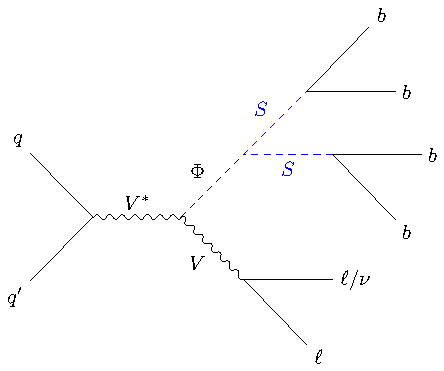
\includegraphics[width=0.33\textwidth]{fig_01a.pdf}}
    \hfill
    \subfloat[ALP模型]{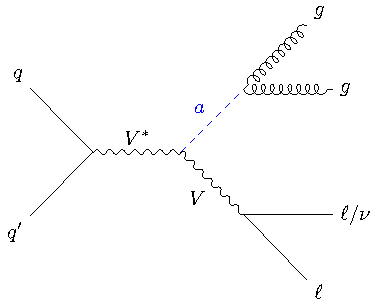
\includegraphics[width=0.33\textwidth]{fig_01b.pdf}}
    \hfill
    \subfloat[暗光子模型]{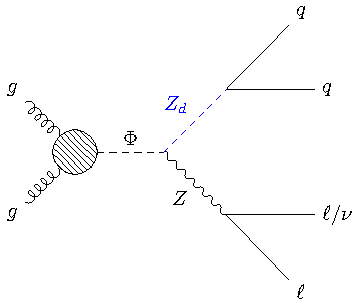
\includegraphics[width=0.33\textwidth]{fig_01c.pdf}}
    \caption{信号模型的费曼图示例\cite{ATLAS:2022zhj}}
    \label{fig:Feynman_diagram}
    \figurenote{
        (a): 隐藏区域模型中介子 $\Phi$ 与矢量玻色子 $V = W$ 或 $Z$ 共同产生,长寿命粒子 $S$ 衰变为费米子(主要为 $b$ 夸克)。
        (b): 类轴轻子(ALP)模型,长寿命粒子 $a$ 衰变为胶子,并与矢量玻色子共同产生。
        (c): 暗光子 $Z_d$ 模型中,$Z_d$ 与 $Z$ 玻色子一同由介子 $\Phi$ 的衰变产生。
    }
\end{figure}

这三种模型的费曼图示例如\autoref{fig:Feynman_diagram} 所示。
对于所有信号样本,生成的 LLP 的平均本征寿命$\tau_{\text{gen}}$是经过选择以最大化其在 ATLAS 强子量能器与 μ 子系统中衰变的事件比例。
这些平均本征寿命通常在几米数量级,但由于时间膨胀效应,不同样本之间有所差异。
每次束团交叉中的堆积背景(pile-up)通过将模拟的硬散射事件与使用 \Pythia{8.186} 生成的非弹性质子碰撞事件叠加进行建模,
所使用的 PDF 为 NNPDF2.3LO,调参为 A3 tune~\cite{ATL-PHYS-PUB-2016-017}。
探测器的几何结构与响应使用 Geant4~\cite{GEANT4:2002zbu} 进行模拟。
ATLAS 标准重建软件被用于模拟数据与真实碰撞数据的重建。

\subsubsection{背景数据}
主要的标准模型背景包括 CalR+2J 通道中的标准模型多喷注事件,以及 CalR+W 和 CalR+Z 通道中的 W/Z+jets、$t\bar{t}$ 和单顶夸克事件。
尽管最终的背景估计使用的是数据驱动(data-driven)方法,但仍需要蒙特卡洛(Monte Carlo)模拟事件来训练机器学习(Machine Learning)判别器并评估某些系统不确定性。

标准模型多喷注样本使用 \Pythia 8.186~\cite{pythia} 在领头阶(Leading Order,LO)精度生成,
采用 A14 参数调节集~\cite{Pythia_tunes} 进行部分子簇射和强子化的计算。
使用的部分子分布函数(Parton Distribution Function,PDF)为 \NNPDF[2.3lo]~\cite{parton_PDF}。
生成的样本依据不同的\pt 范围被记为 \texttt{JZxW},其中 \texttt{x} 随着\pt 的增加从2到12递增,
具体的\pt 范围与产生截面详见\autoref{cpm:MC} 中的\autoref{tab:background_MC}。

包含 W 或 Z 玻色子与喷注的事件使用 \Sherpa[v2.2.1]~\cite{Sherpa} 进行模拟,
最多两个喷注的矩阵元计算精确到次领头阶(Next-to-Leading Order,NLO),
最多四个喷注的为 LO 精度,采用 \textsc{Comix}~\cite{Comix} 和 \OPENLOOPS~\cite{Open_Loops} 库计算,
部分子簇射使用 \Sherpa 默认设置~\cite{parton_shower}。

$t\bar{t}$ 事件的产生使用 \POWHEGBOX[v2]~\cite{POWHEG_BOX} 在 NLO 精度下模拟,
使用 \NNPDF[3.0NLO] PDF 集,并将 \hdamp 参数设为 1.5 倍的顶夸克质量~\cite{ATL-PHYS-PUB-2016-020}。
事件通过 \Pythia[8.230] 与 A14 参数调节集 和 \NNPDF[2.3LO] PDF 集进行部分子簇射和强子化。
$t\bar{t}$ 包含产生的 NLO 截面被修正为 QCD 的 NNLO 理论预测,并包括通过 Top++2.0~\cite{Beneke:2011mq} 所计算的 NNLL 软胶子重求和。

单顶夸克的产生使用 \POWHEGBOX[v2] 在五味方案下的 NLO QCD 精度模拟,使用 NNPDF3.0NLO PDF 集。
为处理与 $t\bar{t}$ 产生的干涉,采用了图移除(diagram-removal)方案~\cite{Frixione:2008yi}。
事件也使用 \Pythia{8.230} 进行簇射与强子化。
其总截面被修正为带有 NNLL 软胶子修正的 NLO QCD 理论预测~\cite{Aliev:2010zk}。


\section{数据处理}
\begin{figure}[ht]
    \centering
    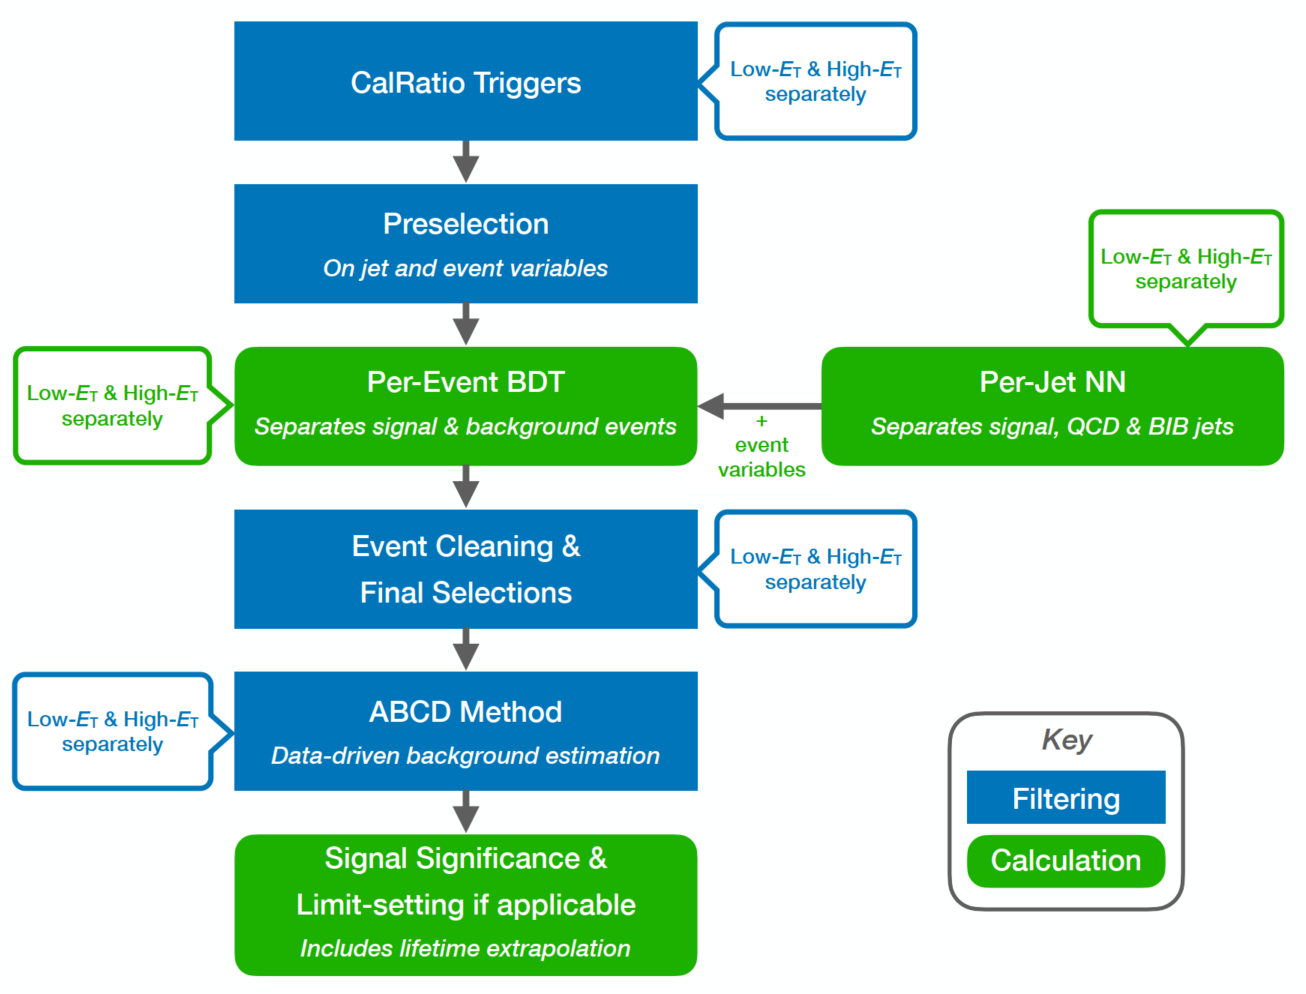
\includegraphics[width=0.85\textwidth]{analysis_strategy.png}
    \caption{分析流程图\cite{ATLAS:2022zhj}}
    \label{fig:analysis_strategy}
\end{figure}

整套分析的流程图如\autoref{fig:analysis_strategy} 所示。
数据通过 CalRatio 触发器进行获取,喷注与事例层级的数据经过预选择之后进入下一步的处理。
对于事件中的每一个喷注,使用了基于深度学习的神经网络(NN)进行分类。
在获得喷注分类的结果后,使用了逐事件的增强决策树(BDT)对事件进行分类。
最终的数据样本是通过对候选事件 BDT 输出值进行选择构建,同时还需满足进一步的数据质量与非对撞背景(NCB)抑制条件,
以确保信号区(Signal Region)具有较高的信号对背景比。
选出的样本被投影到一个二维平面上,其中 $x$ 轴为 $\sum \Delta R_{\min}(\text{jet, tracks})$,
$y$ 轴为逐事件 BDT 的输出值。该平面被划分为四个区域,其中的信号区定义为包含大部分信号且背景贡献预期较低的区域。
为了预测信号区中的背景预期值,使用了基于似然函数的 ABCD 数据驱动方法(又称矩阵法)。
最后对结果进行了极限设定,并将其外推至 LLP 衰变长度在几厘米至 50 米之间的情况。


\subsection{喷注预选择}
\label{sec:jet_preselection}

在本分析中使用的喷注首先通过标准选择进行筛选。
ATLAS 喷注清洗工具所定义的工作点为 \texttt{LooseBad}\cite{ATLAS-CONF-2015-029},
它会排除具有低电磁量能器活性的喷注,导致大多数的信号喷注被消除。
因此,本分析采用工作点 \texttt{LooseBadLLP},该工作点与 \texttt{LooseBad} 的区别在于:
将舍弃低电磁量能器沉积能量比例(low-EMF)喷注的显式条件改为
舍弃 $ |E_{\text{neg}}| > 4~\GeV $ 且 \(\text{FracSamplingMax} > 0.85\) 的喷注。
其中负能量 $E_{\text{neg}}$ 定义为所有具有负能量的量能器单元的能量之和,负能量主要来源于电子噪声和堆叠背景噪声;
FracSamplingMax 为在单一量能器采样层沉积的最大能量占所有沉积能量的比例,

所谓的“clean”喷注需满足以下三个条件:
喷注通过 \texttt{LooseBadLLP} 清洗条件;
喷注的 \(p_T > 40~\GeV \);
喷注的赝快度满足 \(|\eta| < 2.5\)。

\begin{figure}[ht]
    \centering
    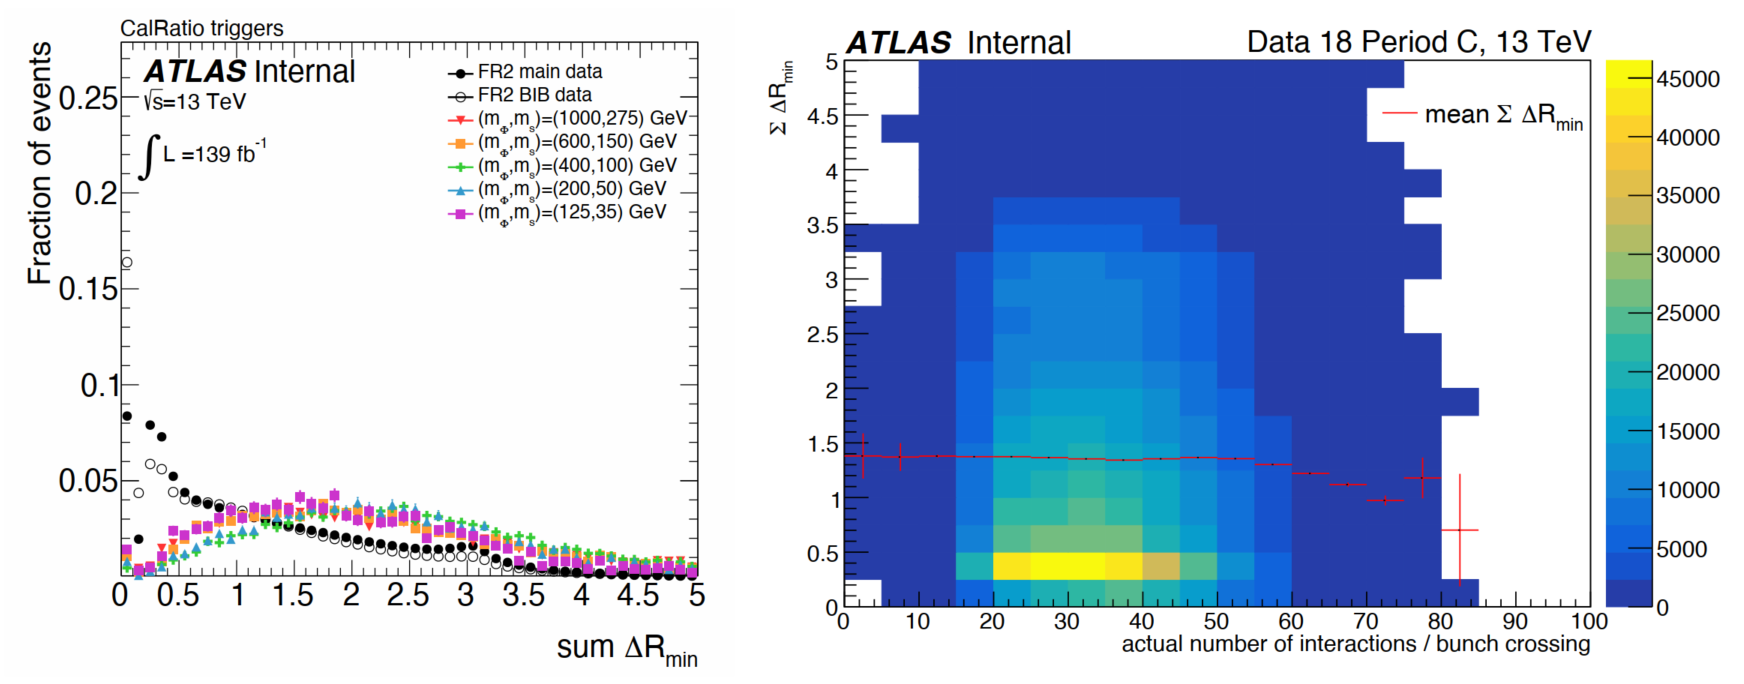
\includegraphics[width=0.95\textwidth]{sumDR.png}
    \caption{$\sum \Delta R_{\text{min}}(\text{jet, tracks})$分布图\cite{ATLAS:2022zhj}}
    \label{fig:sumDR}
    \figurenote{
        左图:预选择之后$\sum \Delta R_{\text{min}}(\text{jet, tracks})$在不同数据集上的分布;
        右图:不同pileup下$\sum \Delta R_{\text{min}}(\text{jet, tracks})$的分布。
    }
\end{figure}

为了选择无径迹喷注的事件,定义了一个事件级变量 $\sum \Delta R_{\text{min}}(\text{jet, tracks})$。
该变量的计算方式为:
对于每个喷注,\(\Delta R_{\text{min}}(\text{jet, tracks})\) 表示该喷注轴线到所有径迹的角距离
$R = \sqrt{(\Delta \phi)^2 + (\Delta \eta)^2}$ 的最小值,同时径迹需满足以下条件:
\begin{itemize}
    \item 径迹满足 \texttt{Charge Pion Loose}\cite{CPgroup} 选择条件;
    \item 径迹与初级顶点兼容,即满足 \texttt{Loose pion-vertex association}\cite{CPgroup} 要求;
    \item 径迹 \(p_T > 2~\text{GeV}\)。
\end{itemize}
随后,将每个 \(p_T > 50~\text{GeV}\) 的 clean 喷注的 \(\Delta R_{\text{min}}(\text{jet, tracks})\) 求和,
得到 \(\sum \Delta R_{\text{min}}(\text{jet, tracks})\) 的值。
该变量对信号事件与标准模型背景事件有良好的区分能力,如\autoref{fig:sumDR} 所示,并且该变量在 pileup 条件下表现出良好的稳定性。
尽管 clean 喷注的定义使用了 \(p_T > 40~\text{GeV}\),
但此处使用 \(p_T > 50~\text{GeV}\) 是因为该阈值在信号与背景的区分上效果最佳。

位移喷注通常是无径迹的,因此其喷注轴线与最近径迹之间的角距离较大。
在含有两个或更多位移喷注的事件中,这些最小角距离的总和也会很大。
如果事件中还存在 prompt 喷注,则其与最近径迹之间的距离会对总和贡献一个较小的量。
相反,在标准模型事件中,大多数喷注周围都有径迹,因此 \(\Delta R_{\text{min}}(\text{jet, tracks})\) 值通常较小。

分析中使用的事件需满足以下预选标准:
至少通过一个 CalRatio 触发器;
至少包含两个 clean 喷注;
\(\sum \Delta R_{\text{min}}(\text{jet, tracks}) > 0.5\)。


% \subsection{提升决策树}
% \label{sec:BDT}

% 需要基于实际数据训练的神经网络(Neural Network,NN)与提升决策树(Boosted Decision Tree, BDT)是鉴别事例是否为信号事例的核心部分。
% 本文的主要工作在于神经网络的设计与实践,关于它的叙述在\autoref{chap:NN}展开,
% 这里着重介绍以逐喷注神经网络输出结果为输入变量的逐事件 BDT。

% BDT 是一种基于集成学习方法的机器学习技术,该方法通过迭代训练多个决策树,
% 每一轮重点关注前一轮难以分类的样本,最终将所有决策树的预测结果通过加权组合,形成一个性能更优的整体分类器。
% 其主要优势在于能够有效提高分类器的准确率;通过调整迭代过程中样本的权重,使模型更关注难分的样本;
% 兼顾多个输入变量,增强对复杂数据模式的捕捉能力。

% 为了将 BIB 事件与至少包含两个具有显著位移喷注的信号事件区分开,设计了一个逐事件 BDT,并使用 HS 模型中的若干组信号样本来对该 BDT 进行训练。
% 训练仅使用事件编号为奇数的事件,而将编号为偶数的事件保留用于最终物理诠释。
% BIB 数据的选取方式如\autoref{sec:detector_data}所述,来自满足 CalRatio 触发器所有高层触发(HLT)条件、但不包括 BIB 抑制算法的数据事件。
% BIB 样本中包含了在造成 BIB 被触发选中的同时叠加的标准模型多喷注事件。因此,即使在训练过程中未显式使用多喷注样本,
% 该逐事件 BDT 也具备区分信号与 BIB 事件以及多喷注背景的能力。

% 高质量($m_\Phi$ = 400 至 1000\,GeV)和低质量($m_\Phi$ = 125 至 200\,GeV)信号样本中的长寿粒子(LLP)通常具有不同的推动(boost),
% 从而导致事件级别上的运动学差异。低质量信号样本中的喷注通常具有比高质量样本更小的横动量$p_\mathrm{T}$,
% 这使得低质量样本与 BIB 的区分更加困难,因为 BIB 喷注具有相对较软的 $p_\mathrm{T}$ 分布。
% 诸如总横动量$H_\mathrm{T}$和有效质量$m_\mathrm{eff}$等事件变量在 BIB 和低质量样本事件中也表现得较为相似。
% 为了在所有信号样本中获得最佳性能,分别训练了两个版本的 BDT:
% 一个在高质量样本中表现更佳(高-$p_\mathrm{T}$ BDT),另一个则更适用于低质量样本(低-$p_\mathrm{T}$ BDT)。
% 这两个训练过程使用了相同的输入变量和 BIB 背景样本,仅在所使用的信号样本方面有所不同。

% 每个事件中的所有 clean 喷注都会通过逐喷注神经网络(per-jet NN)进行评估。
% 在信号数据中,事件中具有最高信号 NN 权重的两个喷注最有可能源自量能器中的 LLP 衰变,
% 这两个喷注被称为 CalRatio 喷注候选,记为 $\text{jet}^{\text{sig1}}$ 和 $\text{jet}^{\text{sig2}}$。
% 在 BIB 数据中,事件中具有最高 BIB NN 权重的两个喷注(BIB 喷注候选)最有可能是 BIB 喷注,
% 记为 $\text{jet}^{\text{BIB}1}$ 和 $\text{jet}^{\text{BIB}2}$。
% 这两类喷注的 NN 输出与其他事件特征一起,作为逐事件 BDT 的输入变量。
% 其余的输入变量的定义可在\autoref{cpm:BDT} 中查阅。

% 此外,$p_\mathrm{T} > 30~\text{GeV}$ 的阈值用于计算 $H_\mathrm{T}$ 和 $m_\mathrm{eff}$ 等变量,
% 这与 clean 喷注所要求的 $p_\mathrm{T} > 40~\text{GeV}$ 阈值不同。
% 这样做的原因是这些变量需要尽可能宽松的选择(同时去除 pileup 产生的软喷注),以便捕捉事件的整体动力学。

% \begin{figure}[ht]
%     \centering
%     \subfloat[低-$p_\mathrm{T}$ BDT]{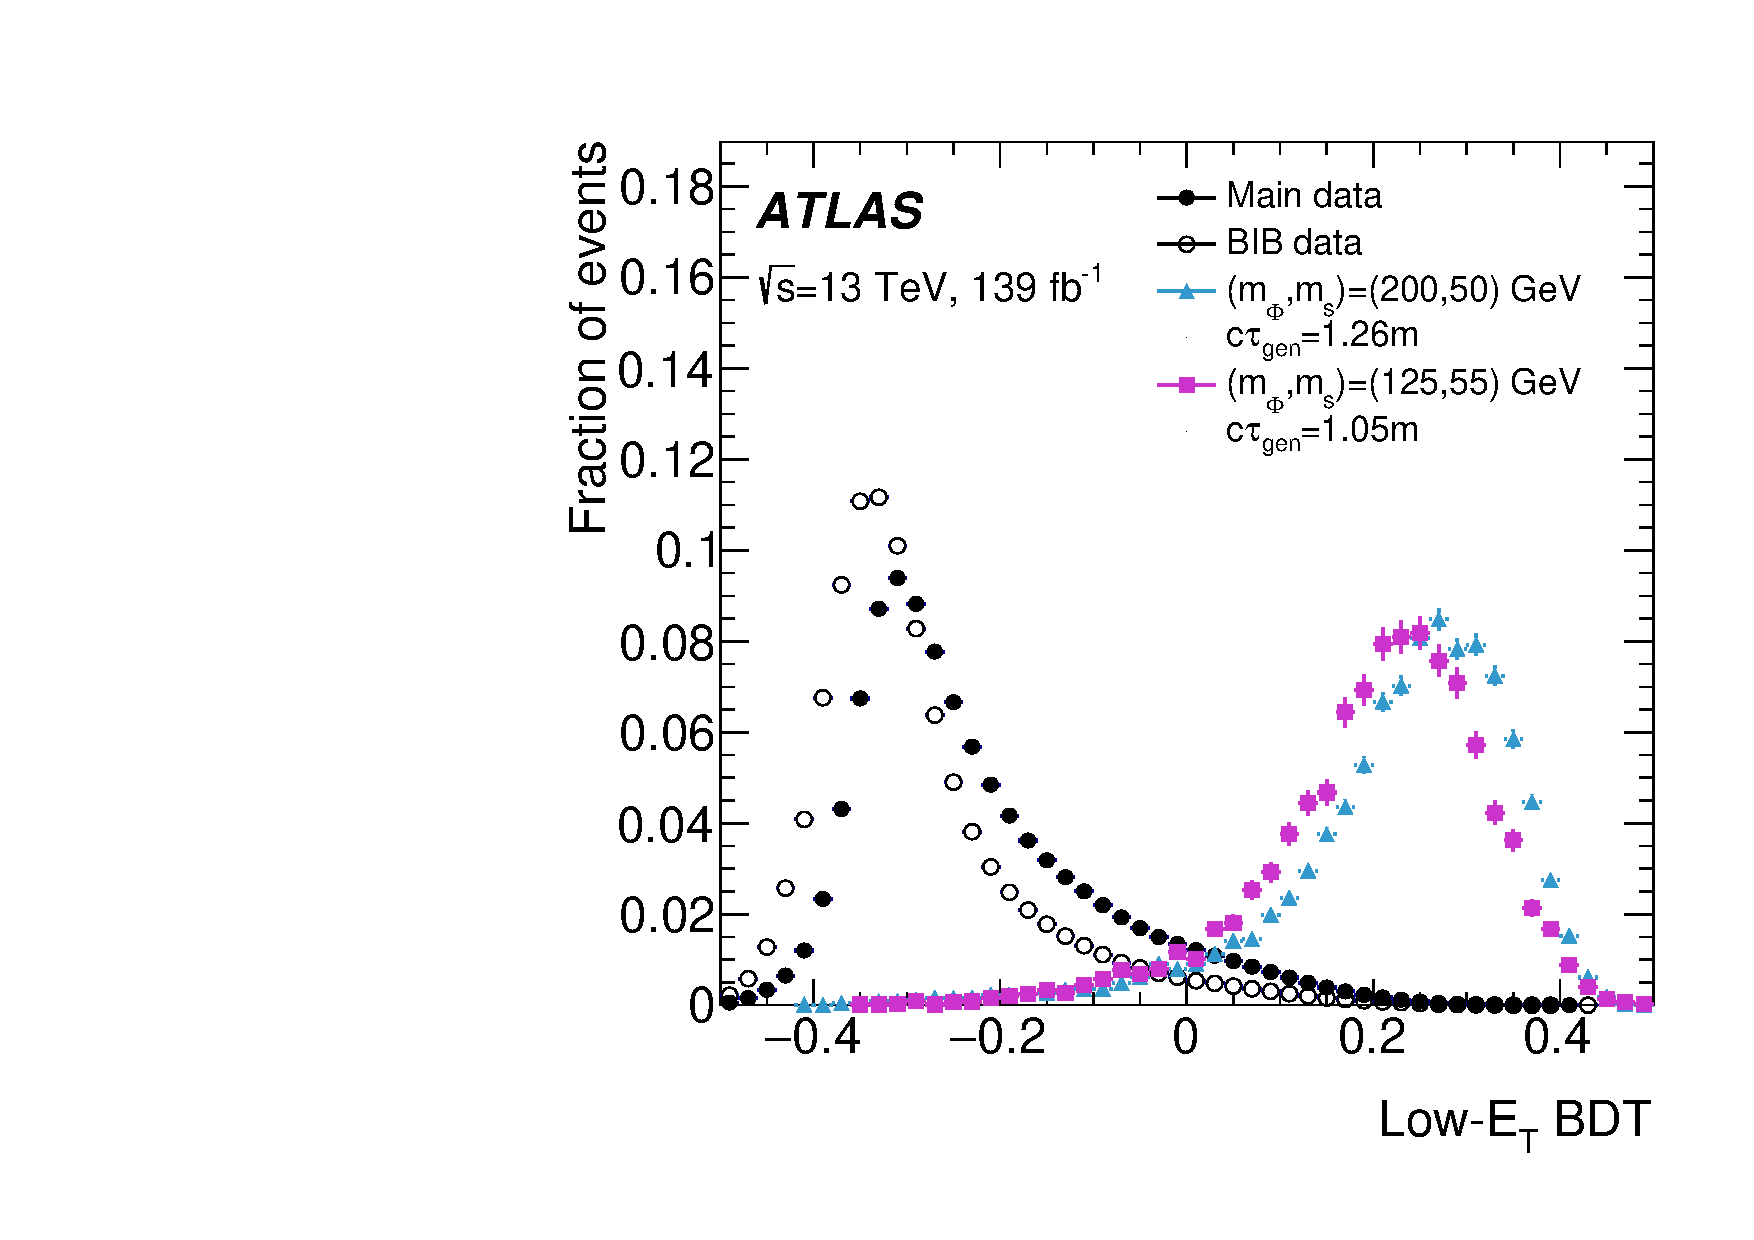
\includegraphics[width=0.45\textwidth]{fig_07a.pdf}}
%     \hfill
%     \subfloat[高-$p_\mathrm{T}$ BDT]{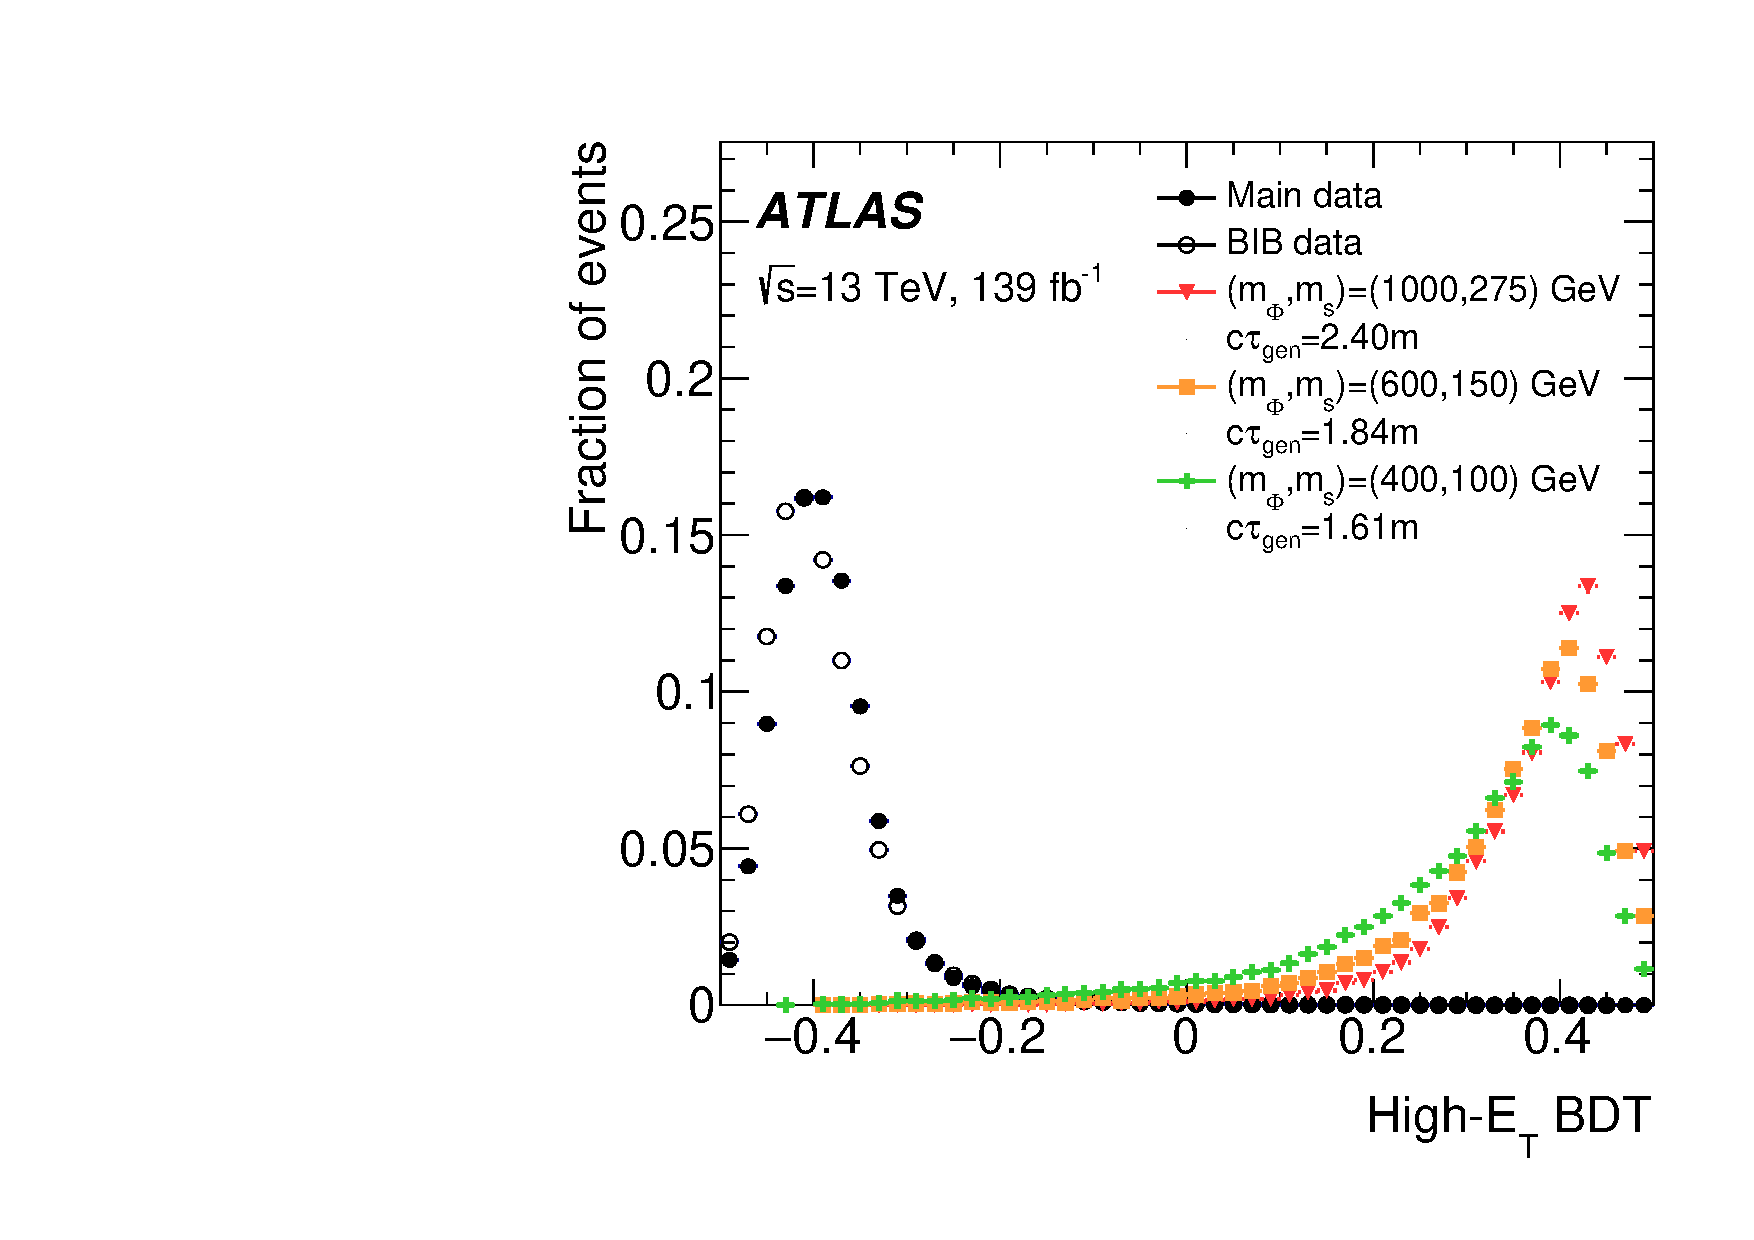
\includegraphics[width=0.45\textwidth]{fig_07b.pdf}}
%     \caption{BDT 在主数据集、BIB数据集、五种信号数据集上的输出分布}
%     \label{fig:BDT}
% \end{figure}

% 两种 BDT 的训练结果见\autoref{fig:BDT},它们的性能均呈现出三个不同区域的结构:
% 极低 BDT 得分区域对应于高 BIB 污染的事件;中间区域主要由 BIB 污染较低的多喷注事件构成;而较高的 BDT 得分区域则对应于信号类事件。
% 考虑到 BIB 与多喷注之间的区分,逐事件 BDT 在本分析中发挥着双重作用:
% 首先,它作为事件清洗的一部分,用于去除 BIB 事件;
% 其次,它与 $\sum \Delta R_\mathrm{min}(\text{jet, tracks})$ 一同构成了定义信号区(Signal Region)的 ABCD 平面的两个变量。


% \subsection{事件清洗}
% \label{sec:Event_Cleaning}

% ABCD 方法用于本分析中的背景估计,其关键是在 ABCD 平面中定义两个不相关的变量。
% 当最终选择中包含多个背景组成部分时,只有在它们在 ABCD 平面上的分布相同时,变量之间的不相关性才得以保持。
% 而在类 QCD 事件与 BIB 事件组合的情况下,这一条件并不满足。
% 因此,控制区域 B、C 和 D 中的 BIB 污染可能会影响该方法的正常运作。
% 因此,在应用 ABCD 方法之前,需要将 BIB 背景从平面中去除。

% \begin{figure}[ht]
%     \centering
%     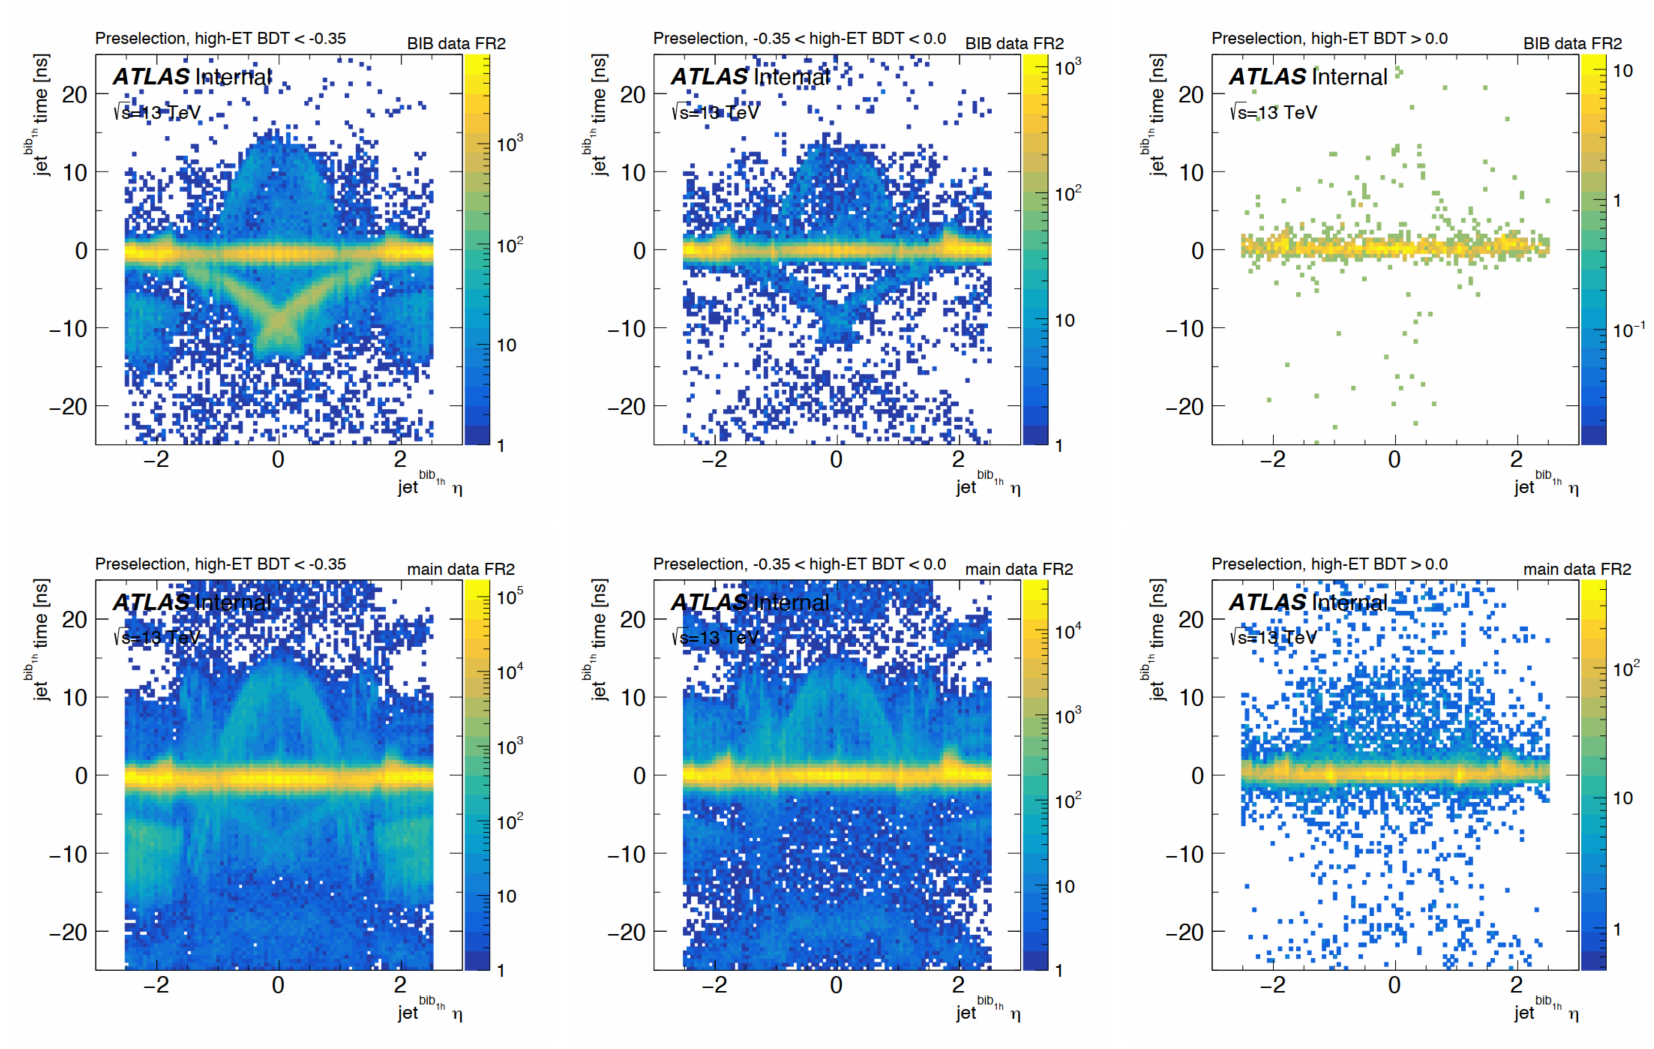
\includegraphics[width=\textwidth]{BIB_eta_time.png}
%     \caption{BIB 候选喷注的$\eta$--$t$分布图}
%     \label{fig:BIB_eta_time}
%     \figurenote{
%         第一行为 BIB 数据集上的结果,第二行为主数据集上的结果。
%         左侧的图为 BDT 得分$< -0.35$的事件;
%         中间的图为 $-0.35 <$ BDT 得分 $< 0$的事件;
%         右侧的图为 BDT 得分 $> 0$的事件。
%     }
% \end{figure}

% \autoref{fig:BIB_eta_time} 展示了 BIB 候选喷注在不同 BDT 得分区间上的$\eta$关于时间的分布。
% 每个图的第一行对应 BIB 样本(以 BIB 为主,并带有少量 multi-jet 污染),第二行为主数据(以 multi-jet 为主,带有少量 BIB 污染)。
% 左侧的图展示了 BDT 得分$< -0.35$的事件,这些事件主要是当前束团交叉中的 BIB,其时间为负值。
% 中间的图为 $-0.35 <$ BDT 得分$< 0.0$的事件,除了当前束团交叉的 BIB 贡献外,还包括下一束团交叉的 BIB,出现在正时间弯曲带中。
% 在此范围内也能看到以 $0$ ns 为中心的 SM 喷注贡献。
% 右侧的图展示了 BDT 得分$> 0.0$的事件,这些事件以 multi-jet 为主,几乎不含时间偏离零的喷注。
% 于是 BIB 的典型形状表现为穿越 $-10$ ns(当前 BC)和 $+15$ ns(下一个 BC)处的弯曲带状结构。
% 因此,进入数据分析的事件被要求满足 BDT 得分$> 0.0$,以确保绝大多数非碰撞背景(NCB)在该阶段已被剔除。

% 在应用预选和上述逐事件 BDT 选择后,仍存在一些事件,其特征既不像多喷注背景,也不像信号。
% 因此,需要进一步的选择来清除这些事件。完整的事件清洗要求如下:

% \begin{itemize}
%     \item BDT 得分$> 0$;
%     \item 触发匹配:至少一个 CalRatio 喷注候选需与触发的 HLT 喷注匹配,
%           匹配定义为 $\Delta R(\text{offline jet}, \text{HLT jet}) < 0.2$;
%           此外,该喷注还需满足 $\log_{10} \text{CalRatio} > 1.2$ 且
%           $\Delta R_{\min}(\text{jet}, \text{tracks}) > 0.2$;
%     \item CalRatio 喷注候选的时间需满足 $-3 < t < 15$ ns。
%           此时间要求用于剔除来自前一个和下一个束团交叉的 pileup,因为其时间主要分布在 $\pm 25$ ns 附近;
%     \item 清洗条件:剔除落入电磁量能器桶部与端盖过渡区域的喷注($1.45 < |\eta| < 1.55$),
%           该区域电磁量能器覆盖不足,会导致伪低 EMF 喷注的产生;
%     \item 探测器噪声及其他效应可能产生具有极低 $\log_{10} \text{CalRatio}$ 的喷注,导致数据与 MC 在该变量上的比较不一致。
%           这一现象在用于研究 ABCD 方法系统不确定性的双喷注控制区中观察到。
%           为避免引入该失拟合区域,且由于这些喷注对本分析不具意义,若任一 CalRatio 或 BIB 喷注候选的
%           $\log_{10} \text{CalRatio} < -1.5$(即 EMF $> 96.9\%$),则不考虑该事件。
% \end{itemize}


% \subsection{最终选择}
% \label{sec:Final_Selection}
